\documentclass{article}
\usepackage{graphicx}
\usepackage{polski}

\usepackage[letterpaper,top=2cm,bottom=2cm,left=3cm,right=3cm,marginparwidth=1.75cm]{geometry}

\usepackage{amsmath}
\usepackage[colorlinks=true, allcolors=blue]{hyperref}

\title{Analiza procentu zwycięstw drużyny NBA na podstawie transferów wykonanych w offseason}
\author{Igor Podgórniak, 272640}

\begin{document}
\maketitle


\section{Wstęp}
\subsection{Wprowadzenie do tematu}
Koszykówka to dynamiczna gra zespołowa, w której dwie drużyny, każda składająca się z pięciu zawodników, rywalizują o zdobycie jak największej liczby punktów, wrzucając piłkę do kosza przeciwnika. Wartość punktów zależy od miejsca, z którego oddano rzut. Poza zdobytymi punktami w koszykówce wyróżnia się inne ważne statystyki:
\begin{itemize}
    \item Zbiórki - sytuacje, w których zawodnik przejmuje piłkę po nieudanym rzucie, czyli po tym, jak piłka odbije się od obręczy lub tablicy.
    \item Asysty - przyznawane zawodnikowi, który poda piłkę do kolegi z drużyny w taki sposób, że ten ostatni zdobywa punkty bez konieczności dodatkowych podań czy dryblingu.
    \item Straty - sytuacje, w których drużyna traci posiadanie piłki na skutek błędów, takich jak niecelne podania, faul ofensywny, przekroczenie linii bocznej lub inne naruszenia przepisów.
    \item Przechwyty - sytuacje, w których zawodnik odbiera piłkę przeciwnikowi, najczęściej poprzez celne i szybkie działanie w obronie.
    \item Bloki - zaliczane, gdy zawodnik udaremni próbę rzutu przeciwnika, dotykając piłki w momencie jej wznoszenia się w kierunku kosza.
    \item Faule - naruszenia przepisów gry, które są popełniane przez zawodników w stosunku do przeciwników.
\end{itemize} Poza wyżej wymienionymi, występuje jeszcze wiele innych, bardziej dogłębnych, którymi jednak nie będziemy się zajmować w projekcie. 
W koszykówce drużyny dzielą się na ligi. NBA to profesjonalna liga koszykówki w Stanach Zjednoczonych, uważana za najlepszą i najbogatszą ligę koszykówki na świecie. Składa się z 30 drużyn podzielonych na dwie konferencje: Wschodnią i Zachodnią, a każda konferencja jest dodatkowo podzielona na trzy dywizje. Podział na konferencje ma znaczenie przede wszystkim podczas sezonu regularnego, ponieważ drużyny klasyfikuje się w konferencjach oraz w fazie playoff, gdzie drużyny rywalizują najpierw w ramach swoich konferencji. \newline
W NBA, podobniej jak w innych sportach występuje tak zwany offseason - okres między zakończeniem jednego sezonu a rozpoczęciem następnego. W tym czasie drużyny mogą dokonywać transferów zawodników, podpisywać kontrakty z wolnymi agentami oraz przygotowywać się do nowego sezonu poprzez treningi i mecze towarzyskie. \newline
NBA wyróżnia się na tle innych lig draftem. Draft NBA to coroczne wydarzenie, w którym drużyny NBA wybierają nowych zawodników spośród graczy z college'ów, lig zagranicznych oraz innych młodych talentów. Jest to główny na pozyskanie przyszłych gwiazd ligi.

\newpage
\subsection{Opis problemu} \label{opis}

Problemem wybranym przeze mnie do badania jest zależność między procentem zwycięstw drużyny w NBA, który jest bezpośrednim czynnikiem wpływającym na pozycję drużyny w konferencji a transferami, które drużyna wykonała przed sezonem, bądź w trakcie trwania poprzedniego sezonu.  Analiza tego problemu może pomóc w pewnym stopniu ocenić zasadność transferów. Celem projektu jest zbadanie zmiany procentu wygranych spotkań przez drużynę w sezonie w stosunku do poprzedniego sezonu na podstawie danych dotyczących:
\begin{itemize}
    \item drużyn: \begin{enumerate}
        \item liczby punktów zdobytych na mecz
        \item liczby asyst zdobytych na mecz
        \item liczby bloków zdobytych na mecz
        \item liczby zbiórek zdobytych na mecz
        \item liczby przechwytów zdobytych na mecz
        \item liczby strat popełnionych na mecz
        \item liczby fauli personalnych popełnionych na mecz
    \end{enumerate}
    \item zawodników: \begin{enumerate}
        \item liczby punktów zdobytych na mecz
        \item liczby asyst zdobytych na mecz
        \item liczby bloków zdobytych na mecz
        \item liczby zbiórek zdobytych na mecz
        \item liczby przechwytów zdobytych na mecz
        \item liczby strat popełnionych na mecz
        \item liczby fauli personalnych popełnionych na mecz
    \end{enumerate}
    \item zmian zawodników w drużynach
\end{itemize} a także stworzenie modelu, który będzie estymował zmianę procentu wygranych drużyny na podstawie zawodników przychodzących i odchodzących z drużyny.


\section{Dane}

\subsection{Źródło i zakres danych}

Dane zostały uzyskane ze strony basketball-reference.com i zawierają informacje na temat statystyk drużyn oraz statystyk graczy. Statystyki drużyn i zawodników są podane na mecz. Dane dotyczące zawodników obejmują sezony od 1989-90 do 2021-22. Dane drużyn obejmują wszystkie lata funkcjonowania zespołów, zapewniając szeroki kontekst historyczny do analizy problemu. Oprócz informacji wymienionych w punkcie 2.1, dane zawierają również niewykorzystane w projekcie informacje takie jak wiek, waga, wzrost zawodników czy informacje dotyczące punktów za 2, za 3 i rzutów wolnych. Każdy wiersz dotyczący statystyk zawodnika zawiera również informację o drużynie, w której dany zawodnik grał w danym sezonie, a wiersze zawierające dane drużyn informację o ilości wygranych i przegranych spotkań.

\subsection{Przetwarzanie wstępne (pre-processing)}

Dane wykorzystywane do konstrukcji modelu posiadały puste komórki, które zostały zastąpione wartościami średnimi obliczonymi na podstawie pozostałych komórek w kolumnie. Na podstawie informacji dotyczących ilości wygranych i przegranych spotkań z pobranych danych, wyznaczono procent wygranych spotkań drużyny w danym sezonie i dodano jako nową kolumnę. Jeśli zawodnik występował w sezonie w więcej niż jednej drużynie, to wybrano drużynę, w której rozegrał większą ilość spotkań, a dane z innych drużyn nie zostały wzięte pod uwagę.

\subsection{Przykładowe dane}

Oczyszczone dane dotyczące zawodników
\begin{figure}[htp]
    \centering
    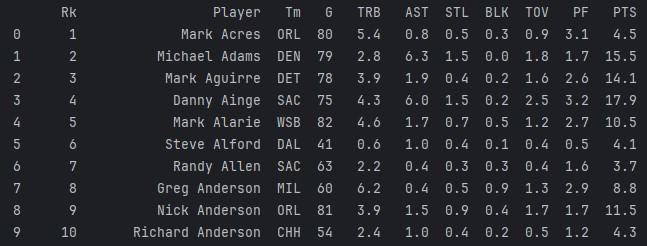
\includegraphics[width=16cm]{merged_players.jpg}
    \label{fig:barplot}
\end{figure}

Oczyszczone dane dotyczące drużyn
\begin{figure}[htp]
    \centering
    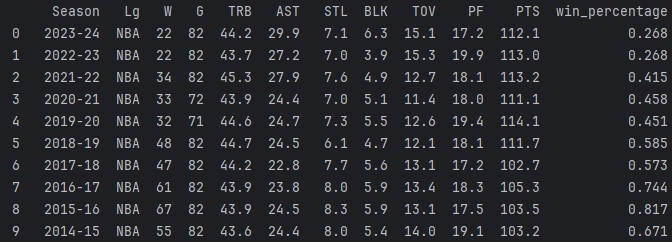
\includegraphics[width=16cm]{cleaned_teams.jpg}
    \label{fig:barplot}
\end{figure}

Dane dotyczące drużyn, wykorzystane w sposobie drugim
\begin{figure}[htp]
    \centering
    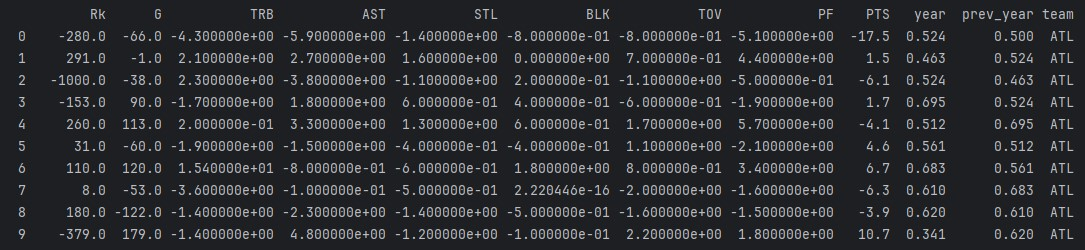
\includegraphics[width=16cm]{merged_data.jpg}
    \label{fig:barplot}
\end{figure}
\newpage


\section{Eksperymenty}

\subsection{Analiza danych}

W celu analizy danych, sprawdzono wpływ statystyk, które będą wzięte pod uwagę podczas późniejszego tworzenia modelu, na wynik drużyny. Do analizy wykorzystano współczynniki regresji liniowej modelu liniowego z biblioteki scikit-learn w Pythonie, na których trenowany był później model.

\begin{figure}[htp]
    \centering
    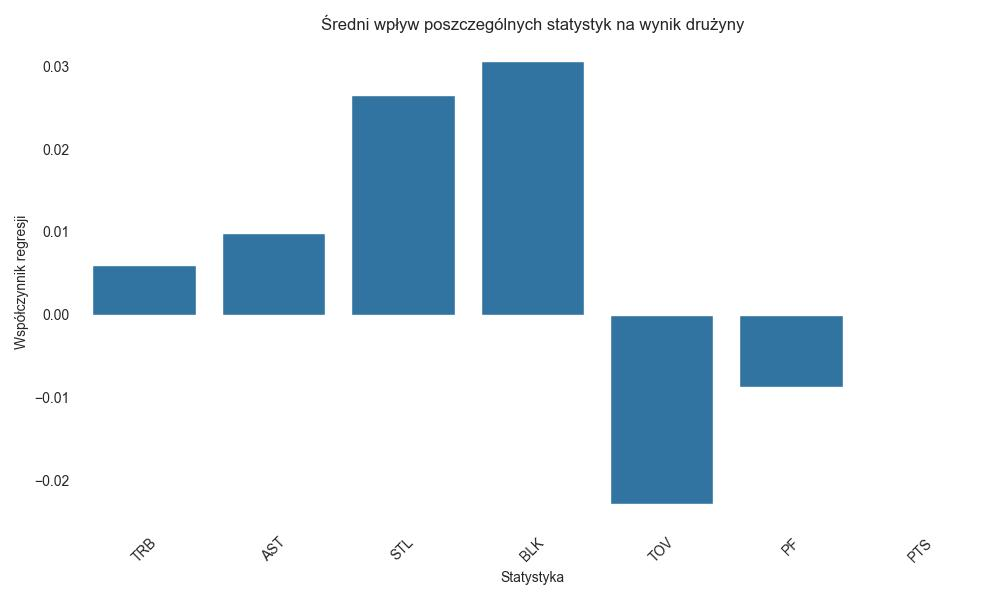
\includegraphics[width=16cm]{barplot.jpg}
    \label{fig:barplot}
\end{figure}

Na wykresie słupkowym przedstawiono wpływ, jaki poszczególne statystyki mają na procent wygranych zespołu w sezonie. Jak widać, największy wpływ na wynik drużyny w sezonie, mają zdobyte bloki i przechwyty, niewielki, ale pozytywny wpływ mają także zbiórki. Straty i faule osobiste wpływają negatywnie na procent zwycięstw. Punkty zdobywane na mecz mają bardzo niski wpływ na wynik zespołu.
\newpage
Te statystyki zilustrowane zostały również za pomocą regresji liniowej:

\begin{figure}[htp]
    \centering
    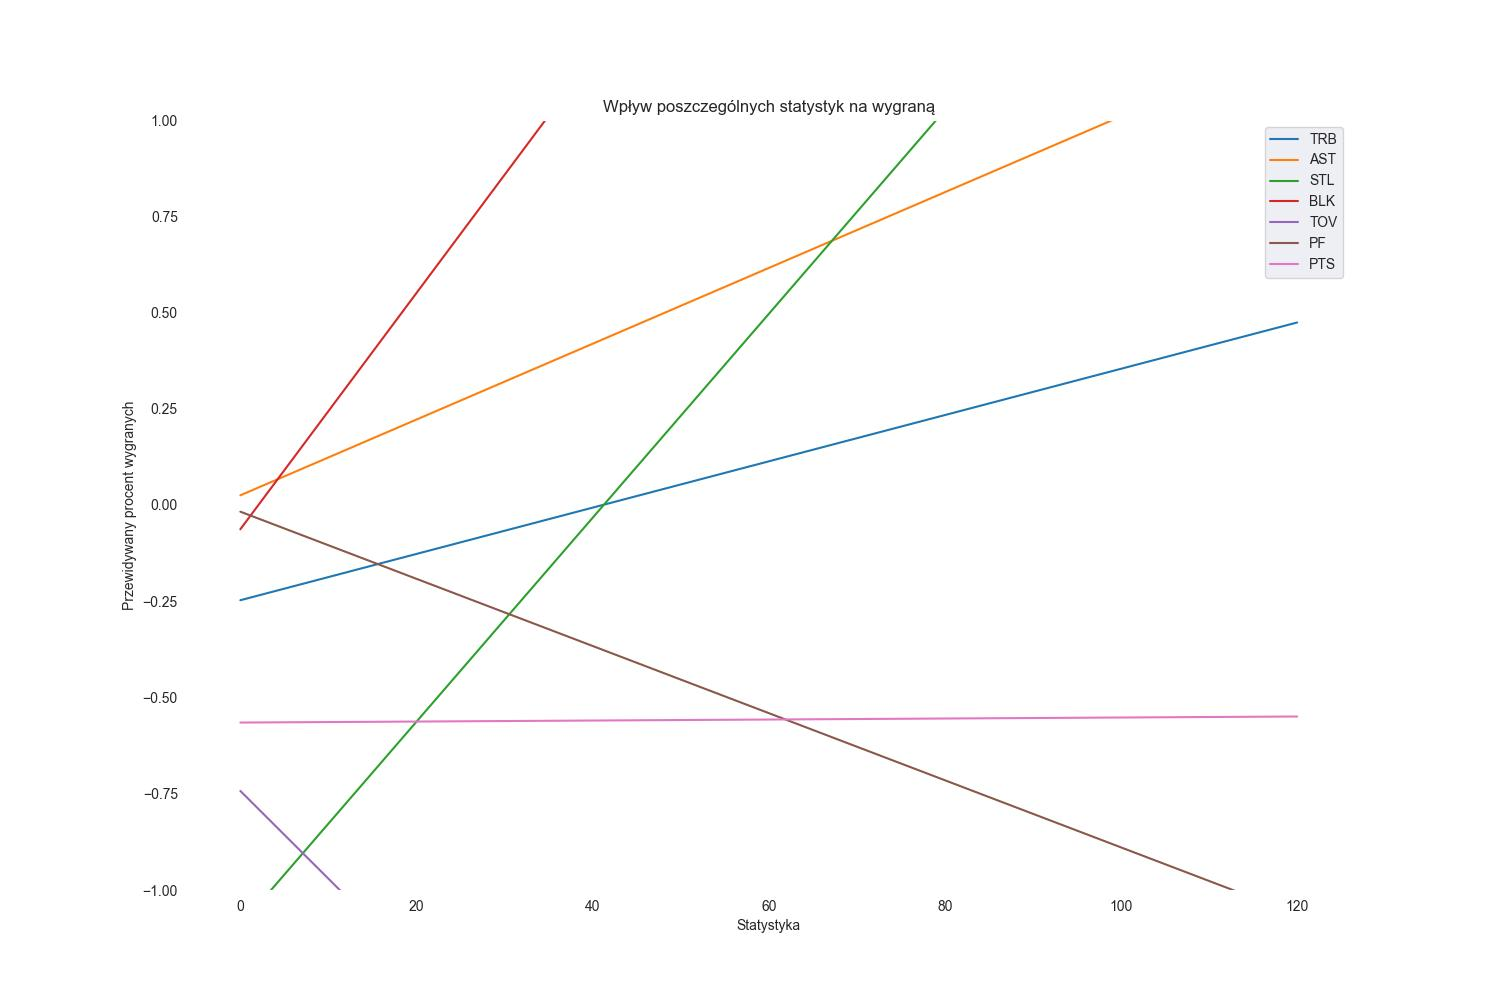
\includegraphics[width=16cm]{reg_analiza.jpg}
    \label{fig:reg_analiza}
\end{figure}

Ten wykresy pokazuje, że mimo dużego pozytywnego wpływu niektórych statystyk na mecz na wynik drużyny w sezonie, ich brak może powodować odmienne skutki, tak jak np. w przypadku przechwytów i zbiórek. Ta zależność działa też w drugą stronę. Przy braku fauli osobistych, ta statystyka nie wpływa na procent wygranych zespołu.
\newpage
Kolejny wykres przedstawia macierz korelacji współczynników regresji poszczególnych statystyk.

\begin{figure}[htp]
    \centering
    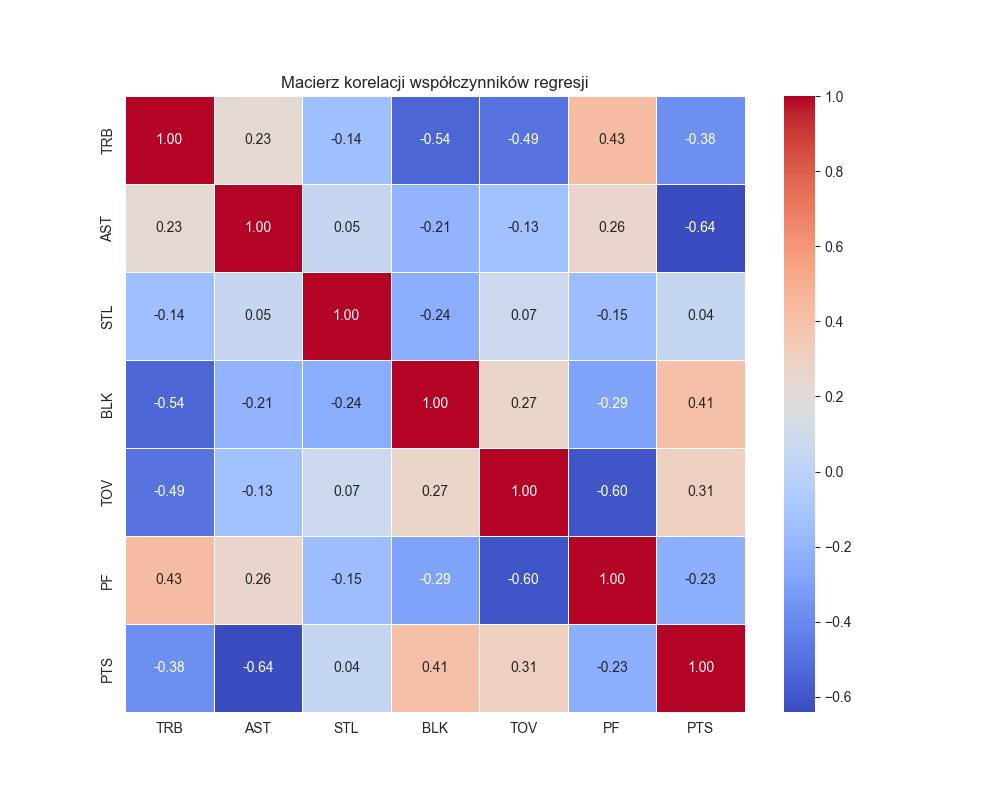
\includegraphics[width=16cm]{corr.jpg}
    \label{fig:corr}
\end{figure}

Na początku należy zaznaczyć, że dane te dotyczą jednej drużyny, nie są oparte na danych meczów i statystykach przeciwników. Na podstawie macierzy, można zauważyć kilka zależności między statystykami. Na pewno interesujący może być związek asyst i punktów na mecz. Zgodnie z danymi, kiedy rośnie liczba zdobytych punktów przez drużynę, zazwyczaj maleje liczba asyst i odwrotnie. Zaskakujący jest też brak większego wpływu liczby przechwytów na zdobywane punkty na mecz. Można także zobaczyć, że wraz z liczbą zbiórek, rośnie liczba fauli wykonywanych przez drużynę, co sugeruje, że walka zbiórki generuje faule.
\newline
\newline
Podsumowując, największą uwagę przykuwa bardzo niski, wręcz niezauważalny wpływ ilości zdobywanych punktów na mecz oraz znaczna przewaga statystyk defensywnych nad ofensywnymi. Te dane potwierdzają przewijającą się w świecie koszykówki tezę, że aktualnie zawodnicy zanidebują defensywną grę ataku, na korzyść większej efektywności w ofensywie. Z tego powodu, samo zdobywanie punktów przez zawodnika, nie ma większego wpływu na przebieg meczu, ważniejsza jest jednak jego skuteczność oraz gra w defensywie. Ponadto negatywne zależności punktów z asystami i zbiórkami w macierzy korelacji, pokazują, że ta statystyka nie ma tak znaczącego wpływu na grę, ponieważ standardem stało się, że drużyny zdobywają podobne, wysokie ilości punktów na mecz.
\newpage


\subsection{Wyniki}


\subsubsection{Sposób 1}
\begin{figure}[htp]
    \centering
    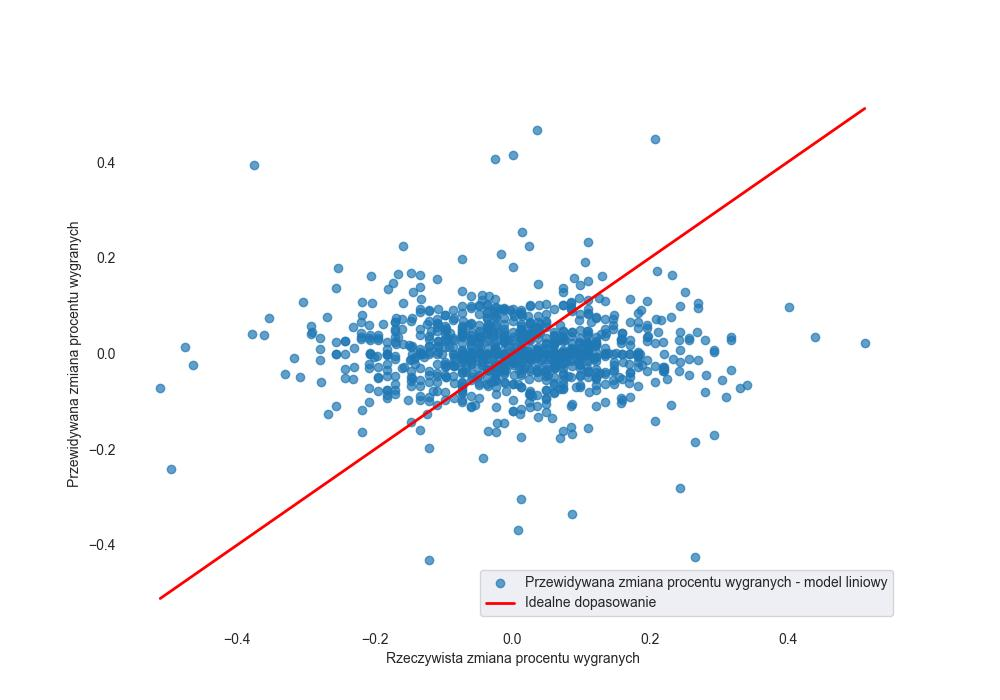
\includegraphics[width=16cm]{linear_model.jpg}
    \label{fig:linear_model}
\end{figure}

W sposobie pierwszym wykorzystano modele użyte wcześniej do analizy danych. Na podstawie ich średnich współczynników regresji wyznaczono wpływ pojedynczego zawodnika na mecz. Następnie znając statystyki graczy, którzy opuścili drużynę i tych, którzy do niej dołączyli, zsumowano wpływ zawodnika z procentem wygranych spotkań drużyny z poprzedniego sezonu i porównano z wartością w poprzednim sezonie. Model regresji liniowej z biblioteki scikit-learn w pythonie przewidywał współczynniki regresji dla każdej zmiennej, które potem były uśredniane dla całej ligi. Najdokładniejsze wyniki znajdują się przy niskich zmianach procentu wygranych.

Obliczono dokładność modelu, wyznaczając jego błąd średniokwadratowy, którego największe wartości osiągały około 0.03. 
\newpage

\subsubsection{Sposób 2}
\begin{figure}[htp]
    \centering
    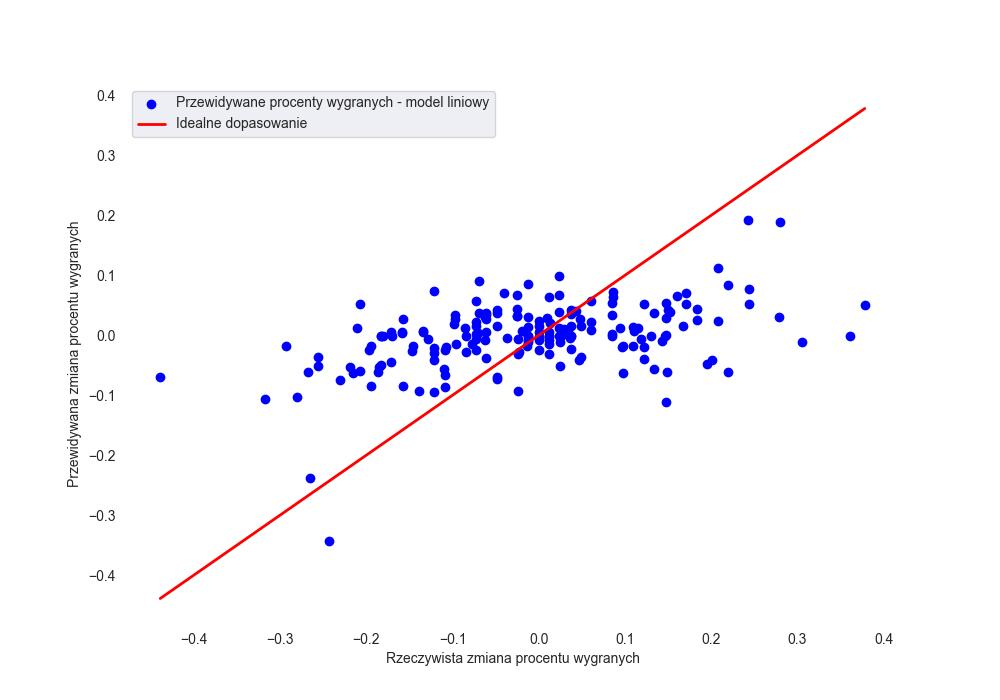
\includegraphics[width=16cm]{linear_model_merged.jpg}
    \label{fig:linear_model_merged}
\end{figure}

W drugim sposobie wykorzystano połączone dane dla wszystkich drużyn w celu wytrenowania modelu bezpośrednio danymi dotyczącymi transferów w offseason i ich wpływu na procent zwycięstw drużyny. Model którego użyto to model regresji liniowej z biblioteki scikit-learn w pythonie. Po kilkunastu uruchomieniach, można zauważyć znacznie mniejszy rozrzut punktów w zależności przewidywanych zmian procentu wygranych od rzeczywistych oraz nieznacznie zmieniony rozkład niż w poprzednim podejściu. Model zazwyczaj przewiduje, że wzrost lub spadek procentu wygranych będzie większy niż rzeczywisty.

Błędy średniokwadratowe modelu przyjmowały wartości w granicach od 0.010 do 0.018.
\newpage

\begin{figure}[htp]
    \centering
    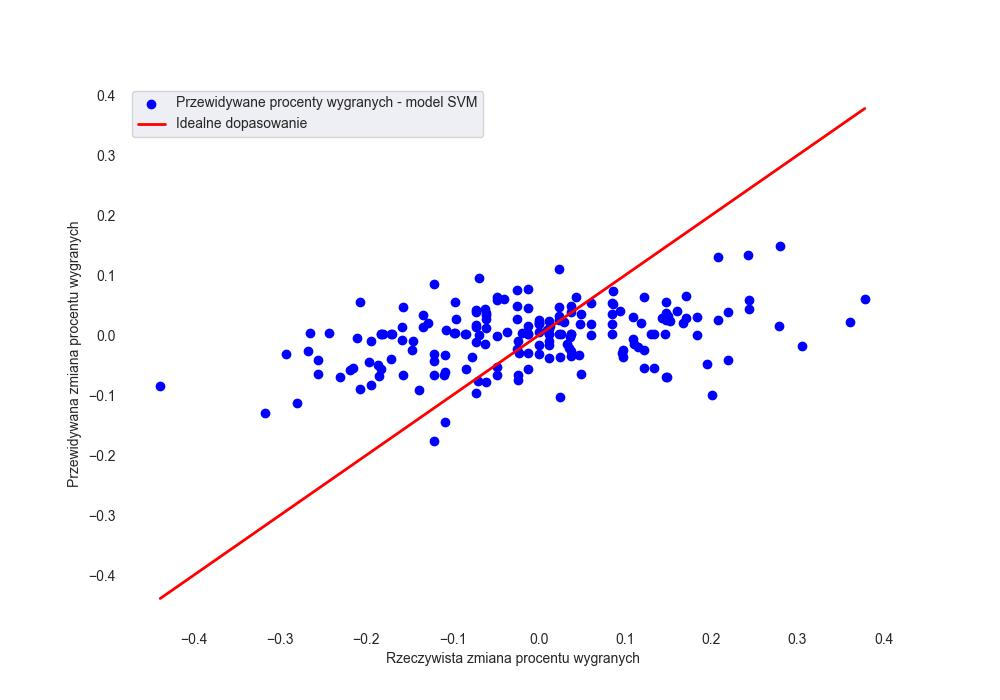
\includegraphics[width=16cm]{svm_model.jpg}
    \label{fig:svm_model}
\end{figure}

Do sposobu drugiego wykorzystano dodatkowo algorytm uczenia maszynowego SVM (Support Vector Machine). Zależność rzeczywistej zmiany procentu wygranych od tej przewidzianej przez model jest tutaj bardzo podobna jak w poprzednim modelu.

Błędy średniokwadratowe w tym modelu przyjmowały bardzo podobne wartości jak w modelu liniowym w sposobie 2.

\subsubsection{Porównanie}

W porównaniu obu metod można zauważyć, że drugi sposób, który bezpośrednio uwzględniał dane dotyczące transferów, osiągnął lepsze wyniki. Modele oparte na danych transferowych wykazały mniejszy rozrzut w przewidywanych zmianach procentu wygranych drużyny oraz mniejszy błąd średniokwadratowy w porównaniu do modeli opartych na analizie statystyk graczy z poprzedniego sezonu.

Wynika to z faktu, że drugi sposób bardziej precyzyjnie uwzględniał specyfikę transferów i bezpośrednio analizował wpływ nowych zawodników na drużynę. Brak pośrednich obliczeń, jak w przypadku pierwszej metody, zmniejszył ryzyko błędów i poprawił dokładność modeli.
\newpage


\subsection{Wnioski}

Na podstawie przeprowadzonych eksperymentów można wywnioskować, że skuteczność transferów w kontekście procentu zwycięstw drużyny w sezonie NBA jest ściśle powiązana z umiejętnościami oraz formą zawodników transferowanych między sezonami lub w trakcie poprzedniego sezonu. Wyniki analizy statystyk graczy z poprzedniego sezonu pokazują, że ich osiągnięcia mają istotny wpływ na przewidywanie efektów ich późniejszych transferów.
\newline
\newline
Analiza danych potwierdza, że statystyki defensywne, takie jak bloki, przechwyty i zbiórki, mają większy wpływ na wynik drużyny w NBA niż statystyki ofensywne, takie jak zdobywane punkty. Negatywny wpływ na procent wygranych mają przede wszystkim straty i faule osobiste, co sugeruje, że skuteczna obrona oraz dyscyplina w grze są kluczowe dla sukcesu drużyny.
\newline
\newline
W obu badanych metodach wykorzystano modele regresji liniowej oraz uczenia maszynowego. Druga metoda, która uwzględniała bezpośrednio dane dotyczące transferów, okazała się skuteczniejsza i dokładniejsza niż pierwsza metoda. Wyniki modeli były bardziej zbliżone do rzeczywistych danych, co sugeruje, że analiza bezpośrednio oparta na danych transferowych może być bardziej efektywna w prognozowaniu zmian procentu wygranych drużyny.
\newline
\newline
Wytrenowane modele mogą być użyteczne dla menedżerów drużyn NBA w podejmowaniu decyzji dotyczących transferów graczy. Mogą one pomóc w przewidywaniu, jakie zmiany w składzie drużyny mogą wpłynąć na jej wyniki w kolejnym sezonie.
Pomimo tego, że modele osiągnęły stosunkowo niskie błędy średniokwadratowe, należy pamiętać, że istnieją inne czynniki, które mogą wpływać na wyniki drużyny, takie jak kontuzje, taktyka gry przyjęta przez trenera, atmosfera w szatni czy forma indywidualnych zawodników. Dlatego też modele te powinny być traktowane jedynie jako narzędzia wspomagające proces podejmowania decyzji.


\end{document}